\frame{\titlepage}

\AtBeginSection[] 
{
  \begin{frame}{What we will know?}
  \tableofcontents[currentsection,hideallsubsections]
  \end{frame}
}
\AtBeginSubsection[]
{
  \begin{frame}{What we will know?}
  \tableofcontents[currentsubsection, hideothersubsections, sectionstyle=show/hide, subsectionstyle=show/shaded/hide]
  \end{frame}
}

{\supressprogressbartrue


\begin{frame}\frametitle{What we will know?}
\tableofcontents[hideallsubsections]
\end{frame}

\supressprogressbarfalse
}

% \begin{frame}
% % \begin{enumerate}
% %     \item Overview and basis
% %         \begin{tikzpicture}[remember picture, overlay]
% %             \draw[decoration={brace}, decorate] 
% %             ([yshift=0.5ex]pic cs:start) --
% %             ([yshift=-2ex]pic cs:end)
% %             node[midway, right=0.3cm] {User level};
% %         \end{tikzpicture}\tikz[remember picture]\coordinate(start);
% %     \item Document creation\tikz[remember picture]\coordinate(end);
% %     \item TikZ and Typography
% %     \item \TeX\ and Typography
% %     \item Command creation
% % \end{enumerate}
     
% %      \begin{itemize}
% %     \item[$\left.\begin{cases}
% %         \text{1.} & \text{First item in the list} \\
% %         \text{2.} & \text{Second item in the list}
% %     \end{cases}\right\}$] Text explaining items 1 and 2
    
% %     \item[$\left.\begin{cases}
% %         \text{3.} & \text{Third item in the list}
% %     \end{cases}\right\}$]
    
% %     \item[$\left.\begin{cases}
% %         \text{4.} & \text{Fourth item in the list} \\
% %         \text{5.} & \text{Fifth item in the list}
% %     \end{cases}\right\}$] Text explaining items 4 and 5
% % \end{itemize}

% % \begin{enumerate}
% %     \item \tikz\node(item1){Item 1};
% %     \item \tikz\node(item2){Item 2};
% %     \item \tikz\node(item3){Item 3};
% %     \item \tikz\node(item4){Item 4};
% %     \item \tikz\node(item5){Item 5};
% % \end{enumerate}

% % \begin{tikzpicture}[overlay, remember picture]
% %     % Bracket for items 1 and 2
% %     \draw[decorate, decoration={brace, amplitude=5pt}, thick]
% %         ([xshift=-5pt, yshift=3pt]item1.north west) -- ([xshift=-5pt, yshift=-3pt]item2.south west)
% %         node[midway, left=12pt] {Group A};

% %     % Bracket for item 3
% %     \draw[decorate, decoration={brace, amplitude=5pt}, thick]
% %         ([xshift=-5pt, yshift=3pt]item3.north west) -- ([xshift=-5pt, yshift=-3pt]item3.south west)
% %         node[midway, left=12pt] {Solo Item};

% %     % Bracket for items 4 and 5
% %     \draw[decorate, decoration={brace, amplitude=5pt}, thick]
% %         ([xshift=-5pt, yshift=3pt]item4.north west) -- ([xshift=-5pt, yshift=-3pt]item5.south west)
% %         node[midway, left=12pt] {Group B};
% % \end{tikzpicture}
% \end{frame}

\section{Technical agreements}

\begin{frame}{Agreements}{I}\relax
     {\Large inclass/outclass versions}
     \begin{itemize}
          \item two slightly different versions for class and home
          \item class version is more interactive and contains less information
          \inclass{\item \inclasshigh{} this line will be shown only in class} 
          \outclass{\item \outclasshigh{} this line will be shown only at home version}
     \end{itemize}
\end{frame}
\inclassframe{\begin{frame}{Frame for a class}
     
\end{frame}}
\outclassframe{\begin{frame}{Frame for home}
     
\end{frame}}

{\supressfootnotefalse
\begin{frame}[fragile]{Agreements}{II}\relax
\newcommand{\tikzmark}[1]{\tikz[overlay,remember picture] \node (#1) {};}

{ \Large Footnotes }
\begin{tikzpicture}[overlay,remember picture]
\draw[->,ultra thick] (0,0.1) to[out=0,in=45] (8, -1.5) to[out=225,in=90] (5,-5.5);
\end{tikzpicture}

\skfootnote{Like this}
\begin{itemize}
     \item For second reading
     \item Contain advanced usage of the command 
     \item Contain references to read more 
     \begin{itemize}
         \item to the exact chapter 
         \item (often) with the href to exact page  
     \end{itemize}
     \item Contains some comments
     \item Mostly for outclass version
\end{itemize}
\end{frame}

}

{\inclassmodetrue
\newcommand{\tikzmark}[1]{\tikz[overlay,remember picture] \node (#1) {};}

\begin{frame}{Agreements}{III}\relax
{ \Large Additional information -- ``magic'' \tikzmark{startM}} 

\begin{tikzpicture}[remember picture,overlay,shift={(current page.north east)}]
\node[anchor=north east,xshift=-0cm,yshift=-0cm](endM) {%
{
\includegraphics[width=1cm]{images/magic}}%
};
\end{tikzpicture}%

\begin{tikzpicture}[overlay, remember picture]
    \draw[->,ultra thick] (startM) to[out=0, in=180] (endM);
\end{tikzpicture}

\begin{itemize}
     \item To have the full picture 
     \item Not to analyze or to puzzle out in class 
\end{itemize}
\end{frame}

}


\begin{frame}{\exFrame{Agreements}}{V}\relax


{ \Large Exercises } 
\begin{tikzpicture}[overlay]
% \draw[white] (0,0) -- (0, 0.6);
\draw[->,ultra thick] (0,0.1) to[out=0,in=-90](-2.1,3.15);
\end{tikzpicture}


\begin{itemize}
     \item To work in class 
\end{itemize}
\end{frame}